%\section{First and Second}
%\chapter{Hardware Implementation} 
\section{Block Diagram} 
Electrical data acquisition and supervision system refer to the process of collecting, monitoring, and analyzing electrical data from various sources to gain insights, detect anomalies, and ensure the proper functioning of our electrical systems. This can be achieved through the use of sensors, data acquisition systems, and monitoring platforms. The design block shown in figure \ref{fig:x System Block}, depicts a complete scenario of our project. 

\begin{figure}[htbp]
\centering
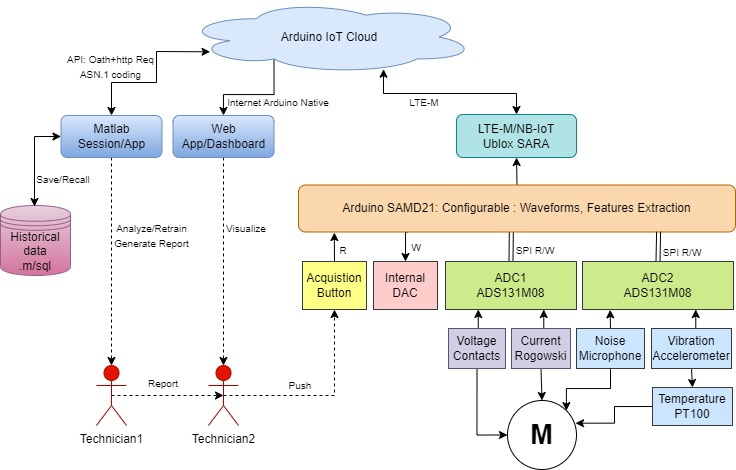
\includegraphics[scale=0.5]{images/Acqsys.jpg}
\caption{ADS131M08 based Acquisition System Block}
\label{fig:x System Block}
\end{figure}

From the figure above, we can observe that this acquisition system can be accessed both manually and via a Matlab session. For the manual option, Technician2 on-site pushes the button. Then, two ADS131M08 ADCs handle the analog data from voltage contacts, current Rogowski sensors, noise, and vibration. The Arduino SAMD21 ARM Cortex M0 processor collects these analog data through SPI communication and sends them to the Arduino IoT cloud using LTE-M. The analog data becomes visible in the cloud, and this acquisition can also be controlled from a push button designed in the cloud. Internal DAC generates analog waveforms for our calibration in house R\&D purpose.
Technician1 can analyze the sample data from the cloud using local Matlab web access. Reading from and writing to the cloud are possible through Matlab web access scripts. Technician1 can also write register values to ADCs via API oath and IoT protocol. For further feature extractions, the RMS calculation algorithm is generated using Simulink, and the resulting C codes can be integrated with the Arduino firmware. 

\section{Arduino MKR NB-IoT} 
In order to provide IoT (Internet of Things) capability combining Narrowband IoT (NB-IoT) and LTE CAT-M1 (LTE-M) communication technologies, Arduino created the Arduino MKR NB 1500, a specialized version of the Arduino MKR family. This gadget combines the capabilities of an Arduino microcontroller with a cellular network to provide cellular network connection to the internet. The pin configuration of an Arduino MKR 1500 has been shown in figure \ref{fig:x Arduino Pinout}. \par
\begin{figure}[htbp]
\centering
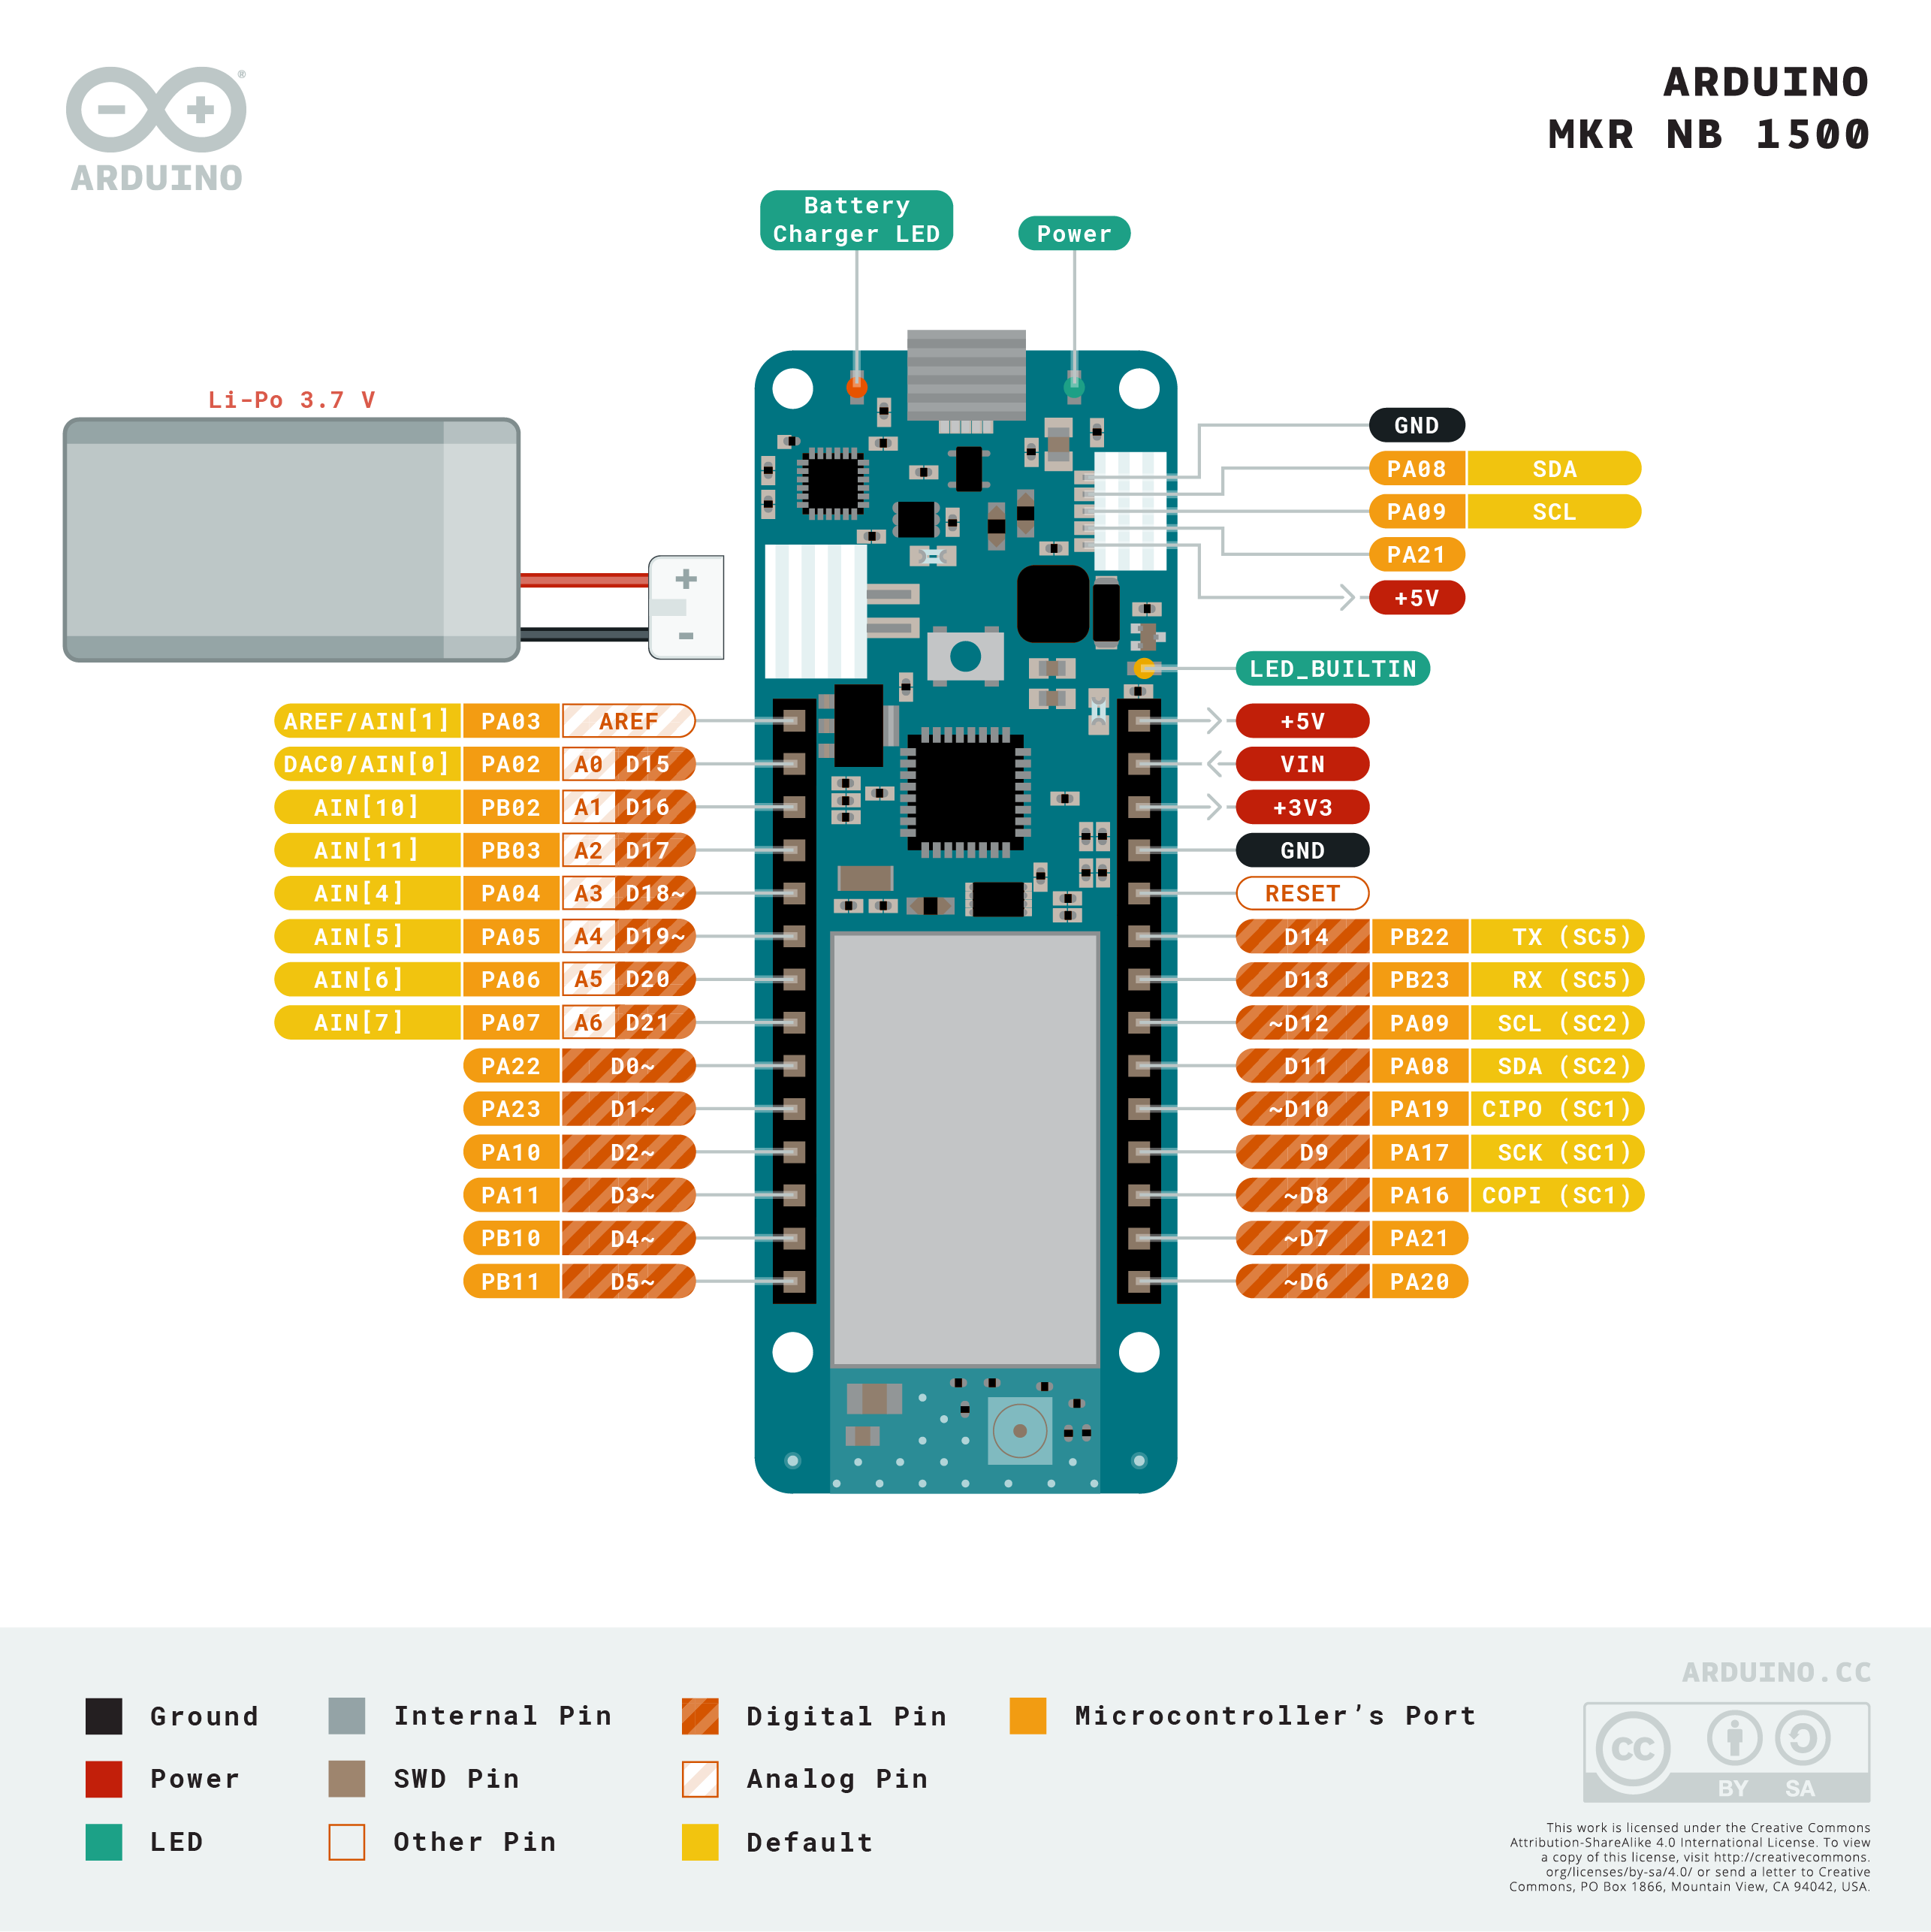
\includegraphics[scale=0.4]{images/Arduino MKR.png}
\caption{Pinout of Arduino MKR NB 1500}
\label{fig:x Arduino Pinout}
\end{figure}
We have selected this board for prototype because of the Key features listed below:\par
\textbf{Communication:} It facilitates communication via LTE CAT-M1 and NB-IoT networks. These are low-power wide-area networks created for Internet of Things (IoT) devices, offering effective and economical data transfer for a range of applications.

\par 
\textbf{Microcontroller:} An ARM Cortex-M0+ microcontroller, which provides computing power and I/O capabilities for communicating with sensors, actuators, and other peripheral devices, is installed on the board.

\par 
\textbf{Integrated SIM Slot:} With an integrated SIM card slot, the MKR NB 1500 makes it simple to connect to the cellular network without the use of additional modules.

\par 
\textbf{Power Management:}The board is designed for low-power operation, making it effective for battery-powered or other power-restricted applications.

\par 
\textbf{Form Factor:} The MKR series boards feature a tiny footprint and a compact form factor, making them ideal for projects with limited space.

\par 
\textbf{Compatibility:} A wide range of I/O pins on the board enable it to interact with a number of sensors, actuators, and other parts frequently used in IoT applications.


\section{ADS131M08 Delta-Sigma ADC} \label{ADS131M08}
Delta-sigma ADCs are commonly used for applications that require high-resolution and high-precision analog-to-digital conversion, such as industrial instrumentation, medical devices, and data acquisition systems. Texas Instruments produces the ADS131M08 analog-to-digital converter (ADC) integrated circuit. In a physical view its a 32 pin ADC shown in figure \ref{fig:x ADS131M08 Chip}. For applications that demand precise and dependable data conversion from analog to digital format, this high-precision, low-power, 24-bit ADC has been developed. All the technical details of this eight channel delta-sigma ADC are available in the Datasheet \cite{ADSDatasheet}. In this section we will discuss some keynote points which were required to configure this ADC.
\begin{figure}[htbp]
\centering
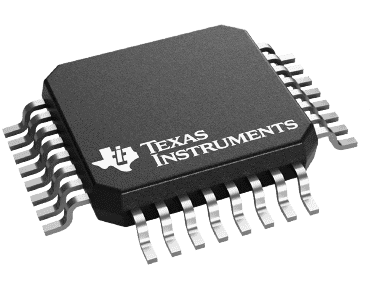
\includegraphics[scale=0.8]{images/ADS131M08 Chip.png}
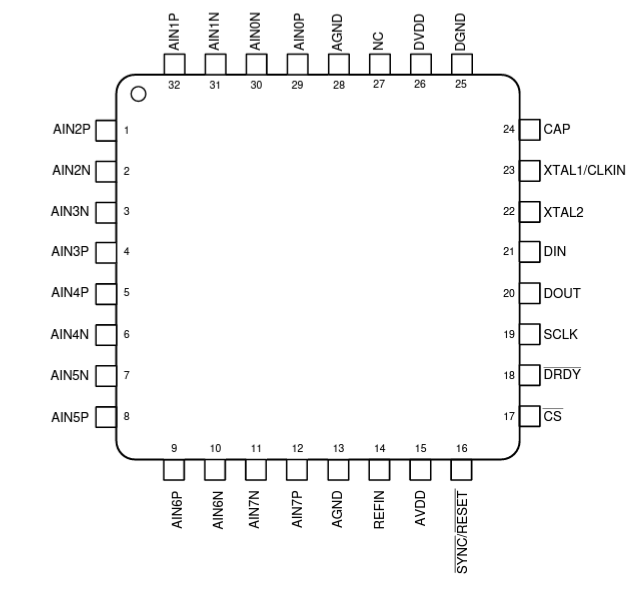
\includegraphics[scale=0.5]{images/pinoutADC.png}
\caption{ADS131M08 Pin  Configuration}
\label{fig:x ADS131M08 Chip}
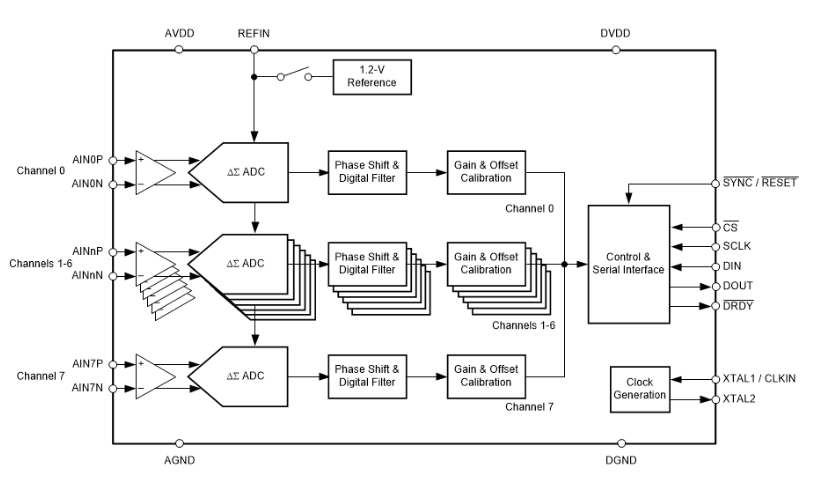
\includegraphics[scale=0.7]{images/Block ADC.png}
\caption{ADS131M08 functional Block}
\label{fig:x ADS131M08 Block}
\end{figure}
Sources for ADS131M08 must be both analog as well as digital. The AVDD-AGND analog source of power may function between 2.7 V and 3.6 V. Absolute input voltages can be as low as 1.3 V below AGND thanks to an incorporated negative charge pump, allowing single-ended power supplies to be used for measurements of input signals that fluctuate around ground. Both 1.8-V and 3.3-V sources are accepted by the digital power supply (DVDD - DGND). A PGA (programmable gain amplifier) with gains of up to 128 is a feature of the gadget. High input impedance is guaranteed at high PGA gain levels via an incorporated input precharge buffer active at gains larger than 4. An inbuilt 1.2-V reference provides the ADC with its reference voltage.Designers can choose between power consumption and ADC dynamic range using three power-scaling options. 
\vspace{1\baselineskip}\par 
The output of the modulators is demodulated by a digital decimation filter that is included into each channel of the ADS131M08. In high-resolution mode, the filter allows data rates of up to 32 kSPS per channel. A precise correction for the sensor phase responses is made possible by the ability to set the relative phase of the samples between channels. It is possible to configure offset and gain calibration registers to automatically correct output samples for detected offset and gain faults. The ADS131M08's functional block diagram in figure \ref{fig:x ADS131M08 Block} offers a thorough illustration of the device. A serial programming interface (SPI) compliant interface is used by the device for communication. The ADS131M08 is managed through a number of internal registers and SPI instructions. 
\vspace{1\baselineskip}\par 
\textbf{PGA:}  \par
 PGA refers to an electronic amplifier that allows the user to adjust its gain (amplification factor) according to their needs.The ADS131M08 has a built-in programmable gain amplifier (PGA) for each channel that offers gains of 1, 2, 4, 8, 16, 32, 64, and 128. The PGAGAINn bits for every channel in the GAIN1 register separately regulate the gains for the various channels. The differential full-scale input voltage range (FSR) of the ADC is scaled by changing the PGA gain. The link between FSR and gain is shown in equation \ref{eqn}. This Equation employs 1.2 V as the internal reference voltage as the scaling factor without taking into consideration gain error brought on the reference voltage tolerance.
\begin{align} \label{eqn}
    FSR = \pm 1.2 V / Gain
\end{align}
\textbf{Voltage Reference:}  \par
An internal and an external reference are the two voltage-reference choices available for the ADS131M08. The reference for the ADC is supplied by the internal reference using a low-drift band-gap voltage. The differential input voltage can range from -1.2 V to 1.2 V since the internal reference has a nominal value of 1.2 V. 
\vspace{1\baselineskip}\par 
\textbf{Clocking and Power Mode:}  \par
A crystal must be attached between the XTAL1/CLKIN and XTAL2 pins in order for the onboard oscillator to create the master clock whether internally or externally through the CLKIN pin.  The serial data clock (SCLK) must be synchronized with the modulator sampling clock for best performance.Since the master clock is the source of the modulator sampling clock, the master clock and SCLK must be in synchronization.  Therefore, for optimum performance, ensure that data retrieval is synchronized to the clock signal at CLKIN and supply a master clock to CLKIN.The device may be set up in any of the all three power modes: high-resolution (HR), low-power (LP), or very low-power (VLP), thanks to the PWR[1:0] bits in the CLOCK register. The internal bias currents are scaled to reach the desired power levels by changing the PWR[1:0] bits.

 
\vspace{1\baselineskip}\par 
\textbf{Delta-Sigma Modulator:}  \par
The conventional input voltage is converted to a one's density modulated digital bit-stream by the ADS131M08 using a delta-sigma ($\Delta\Sigma$) modulator. The ($\Delta\Sigma$) modulation circuit oversamples the supplied voltage at a frequency that is several times higher than its final data rate. The ADS131M08's modulation frequency, $f_{MOD}$, is equivalent to halves of the master clock frequency, or $f_{MOD} = f_{CLKIN} / 2$

\vspace{1\baselineskip}\par 
\textbf{Digital Filter:}  \par
The bitstream from the $\Delta\Sigma$ modulation is fed into the digital filter. The digital filter reduces the out-of-band noise caused by quantization of the modulator and is a linear phase, finite impulse response (FIR), and low-pass sinc-type filtering. By averaging, the digital filter demodulates the $\Delta\Sigma$ modulator's outputs. To decrease the rate at which data exit the modulation unit ($f_{MOD}$) and reach the output data stream ($f_{DATA}$), the data flowing through the filter is downsampled and shredded. Equation \ref{OSReqn} defines the decimation factor, which is also known as the oversampling ratio (OSR).
\begin{align} \label{OSReqn}
    OSR = f_{MOD}/f_{DATA}
\end{align}
The OSR[2:0] entries in the CLOCK register control the OSR and modify it. The ADS131M08 has OSR options that enable various data rate configurations for any specific master clock frequency. For the specified notional CLKIN frequencies, Table \ref{tab:OSR} gives the OSR parameters and their respective output data rates. There are three different types of power mode of this ADC. We have configured it to the Very Low Power (VLP) mode by providing 2.048 MHz clock frequency, and output data rate was 1 ksps.
\begin{table}[htbp]
  \centering
     \caption{OSR Settings and Data Rates}
    \label{tab:OSR}
  \begin{tabular}{|c|c|c|c|c|}
    \hline
    \multicolumn{1}{|c|}{\textbf{Power Mode}} & \multicolumn{1}{|c|}{\textbf{Clock}} & \multicolumn{1}{|c|}{\textbf{$f_{MOD}$}} & \multicolumn{1}{c|}{\textbf{OSR}} & \multicolumn{1}{c|}{\textbf{O/P Data}} \\
    \hline
    \multirow{8}{*}{VLP} & \multirow{8}{*}{2.048 MHz} & \multirow{8}{*}{1.024 MHz} & 128 & 8 KSPS \\
    & & & 256 & 4 KSPS \\
    & & & 512 & 2 KSPS \\
    & & & 1024 & 1 KSPS \\
    & & & 2048  & 500 SPS \\
    & & & 4096 & 250 SPS \\
    & & & 8192 & 125 SPS \\
    & & & 16384 & 62.5 SPS \\
    \hline
  \end{tabular}

\end{table}

\section{Schematic Diagram} 
The schematic shown in figure \ref{fig:x Schematic} has been designed in KiCad software. There are several portions of this schematic which has been listed below:
\begin{figure}[htbp]
\centering
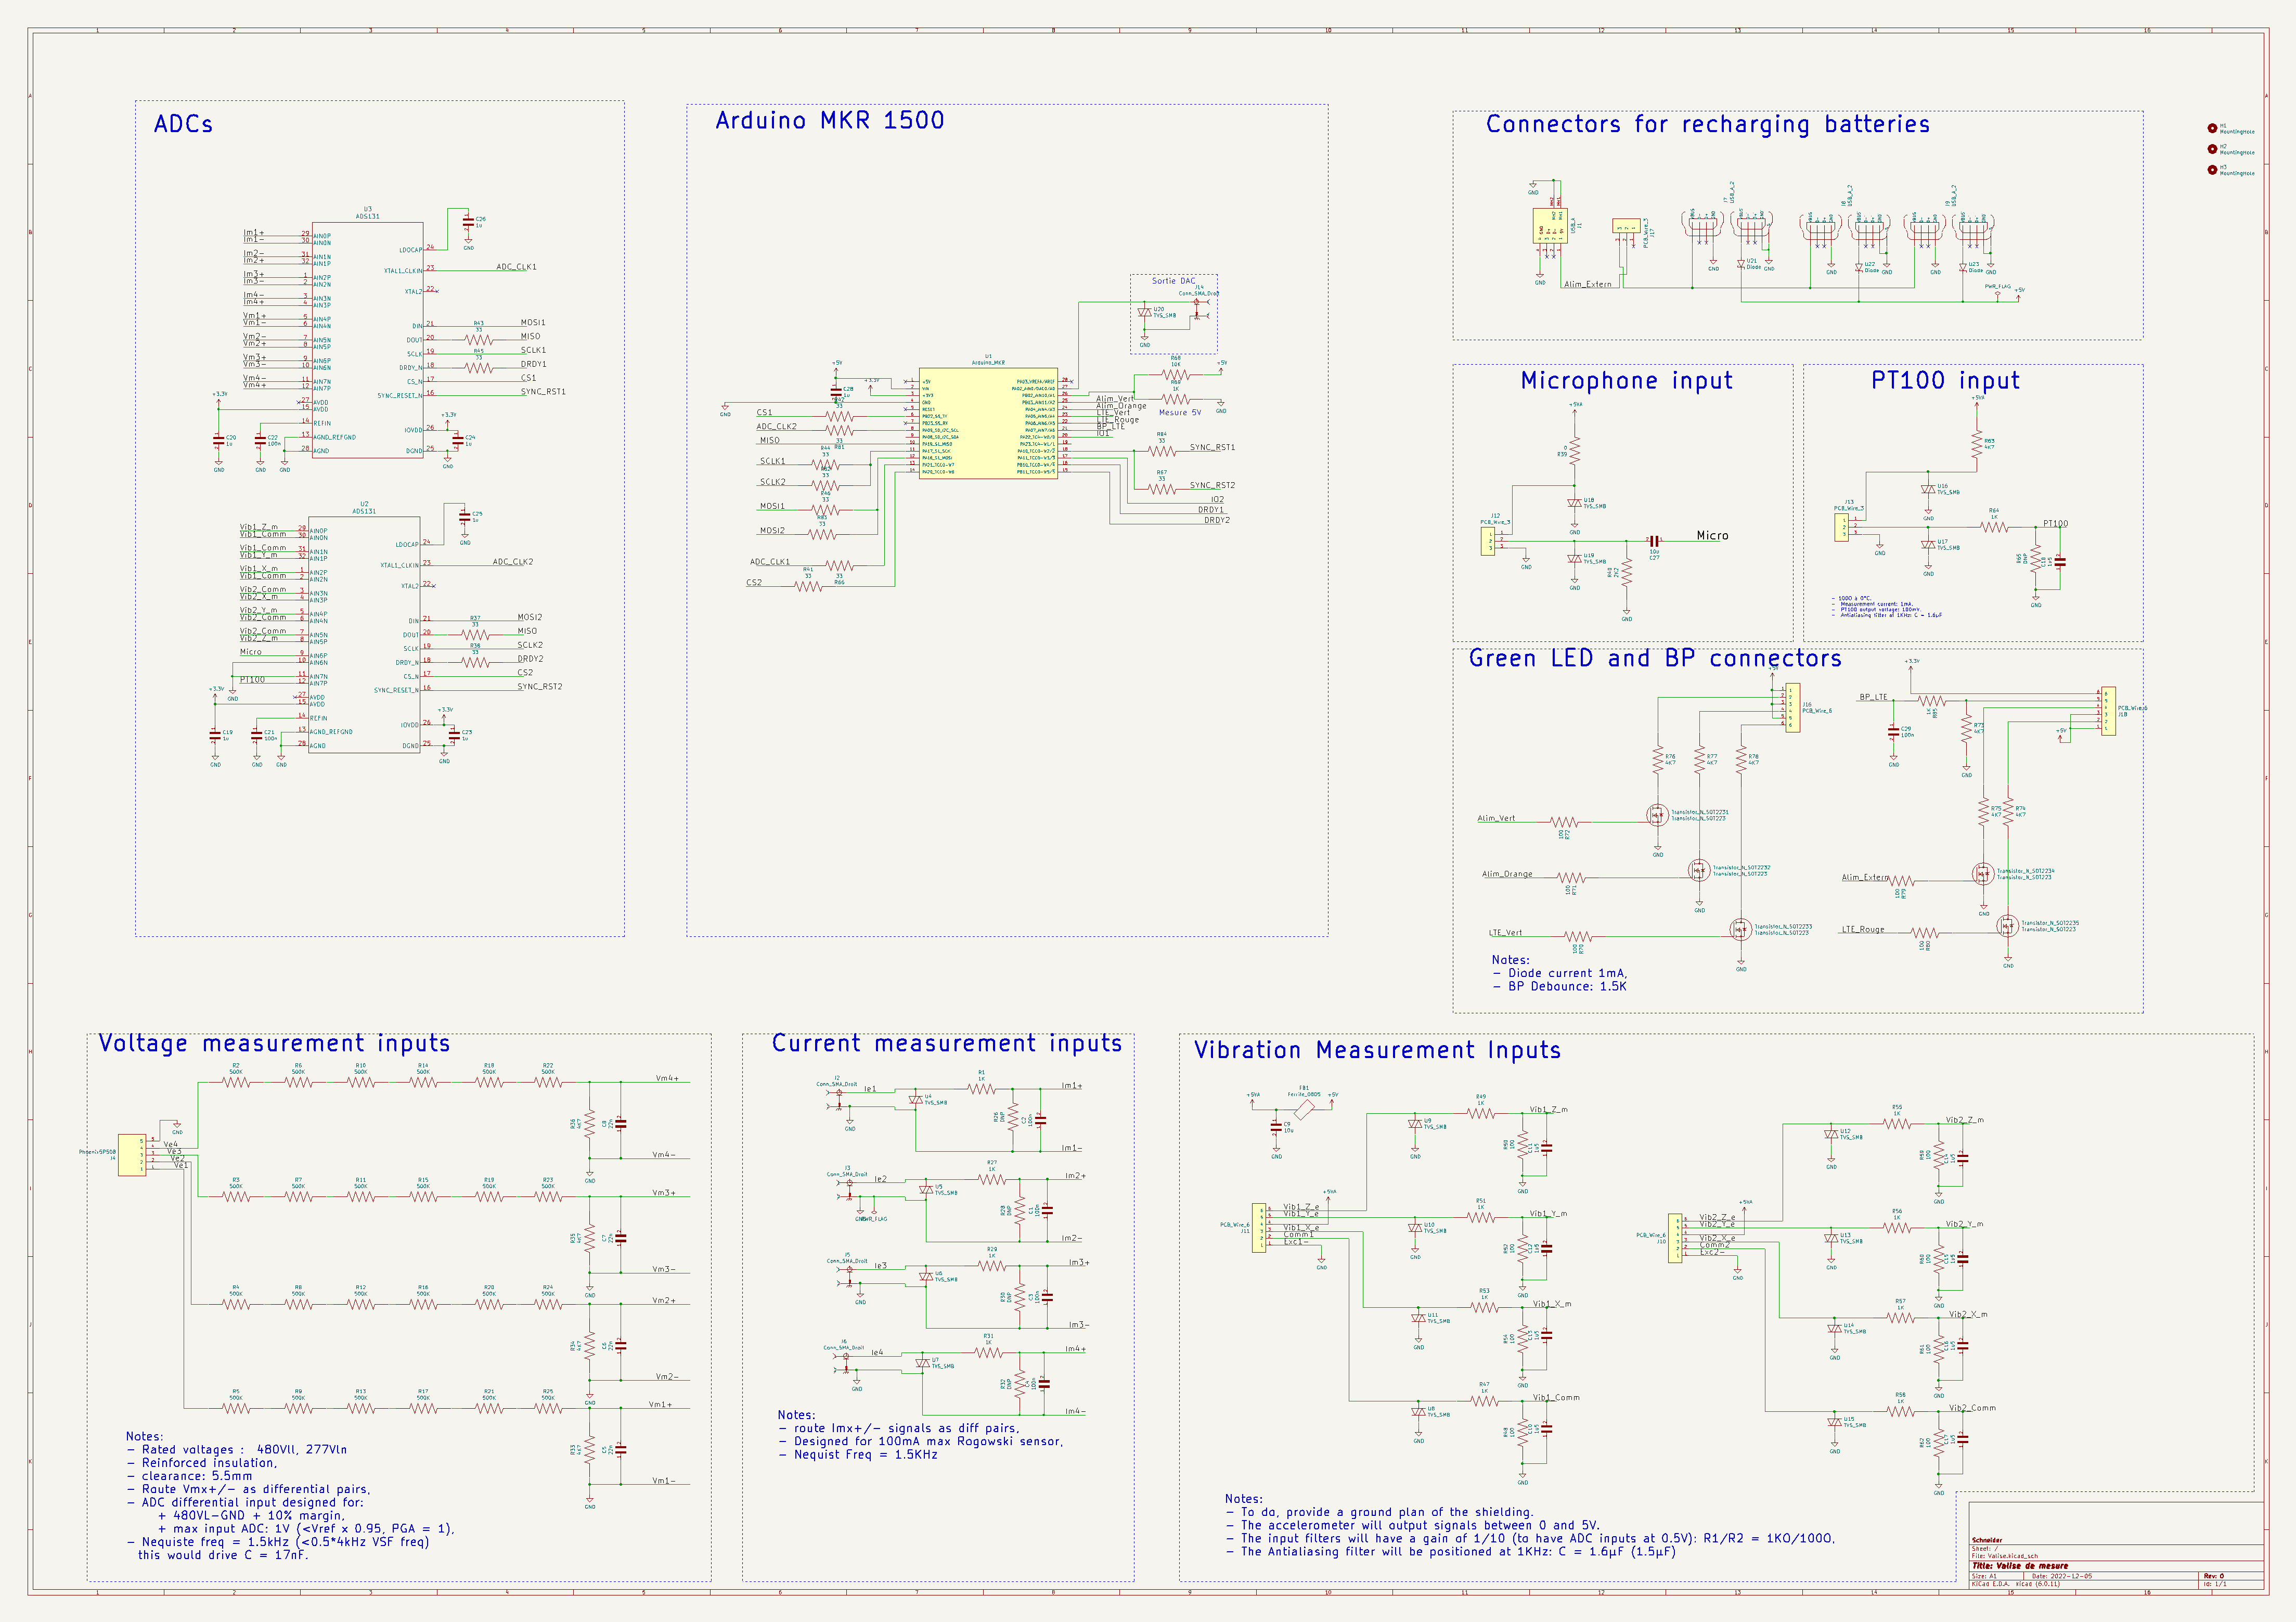
\includegraphics[scale=0.18]{images/Schematic.png}
\caption{Schematic Diagram}
\label{fig:x Schematic}
\end{figure}

\begin{itemize}
\begin{multicols}{2}
  \item Arduino MKR 1500
  \item Two ADCs
    \item PT100 Input
  \item Green LED \& Push Button 
  \item Microphone Input
  \item Voltage Measurement Input
  \item Current Measurement Input
  \item Vibration Measurement Input
   \item Connection for Recharging Batteries
\end{multicols}
\end{itemize}







\section{Printed Circuit Board Assembly} 

The PCBA process is a crucial stage in electronic manufacturing and requires careful attention to detail and quality control to ensure reliable and functional electronic products. Printed Circuit Board Assembly (PCBA) refers to the process of attaching electronic components onto a printed circuit board (PCB) to create a functional electronic circuit.This PCBA process typically involves the following steps:
\par
\textbf{PCB Fabrication: } 
 First, the bare PCB is manufactured by etching copper traces onto an insulating substrate according to the design specifications. The PCB layout is designed using specialized software and contains the necessary traces, pads, and vias to connect the components. We have designed our PCB in KiCad software shown in figure \ref{fig:x PCB design}, and fabricated it from a third party PCB manufacturer.\par
\begin{figure}[htbp]
\centering
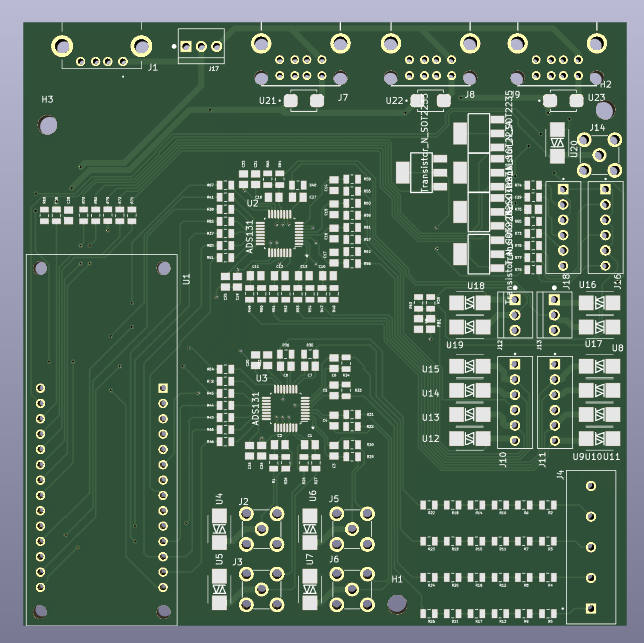
\includegraphics[scale=0.55]{images/Valise.png}
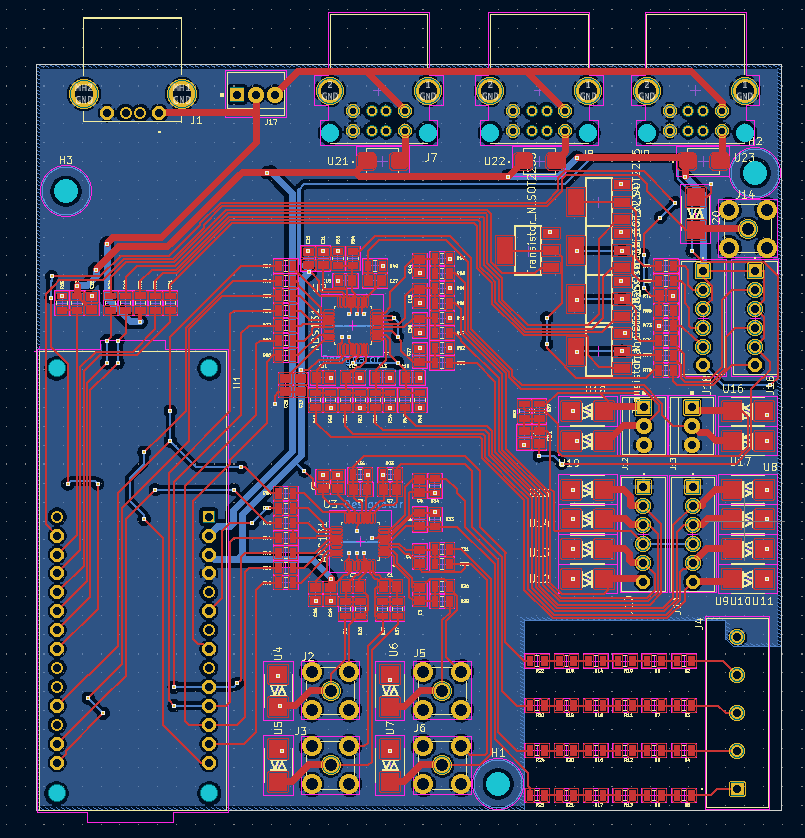
\includegraphics[scale=0.42]{images/PCB Valise.png}
\caption{PCB design of Acquisition System}
\label{fig:x PCB design}
\end{figure}

\textbf{Component Placement:}  
Once the PCB is ready, the electronic components (such as resistors, capacitors, integrated circuits, connectors, etc.) are placed onto the board in their designated locations. There are two main methods for component placement:
\par
\textbf{a. Manual Assembly:}  
 Smaller scale productions may involve manual placement of components. Skilled technicians use pick-and-place machines or soldering irons to carefully position each component.In Schneider's Lab we have implemented our board through manual assembly. Majority of the components on our board were SMD, including the ADC, which made this task quite challenging to overcome precisely.
\par
\textbf{b. Automated Assembly:}  
 For larger-scale production, robotic pick-and-place machines are used to automate the component placement process. The machine picks components from reels or trays and accurately places them onto the PCB based on the design data. In the future, we may consider employing this technique for mass production.
\par
\textbf{Soldering: }  
After the components are placed, they need to be permanently attached to the PCB. Soldering is the most common method for creating these connections. Weller WX 2021 SMD soldering station has been used for the soldering of our PCB.
\par
\begin{figure}[htbp]
\centering
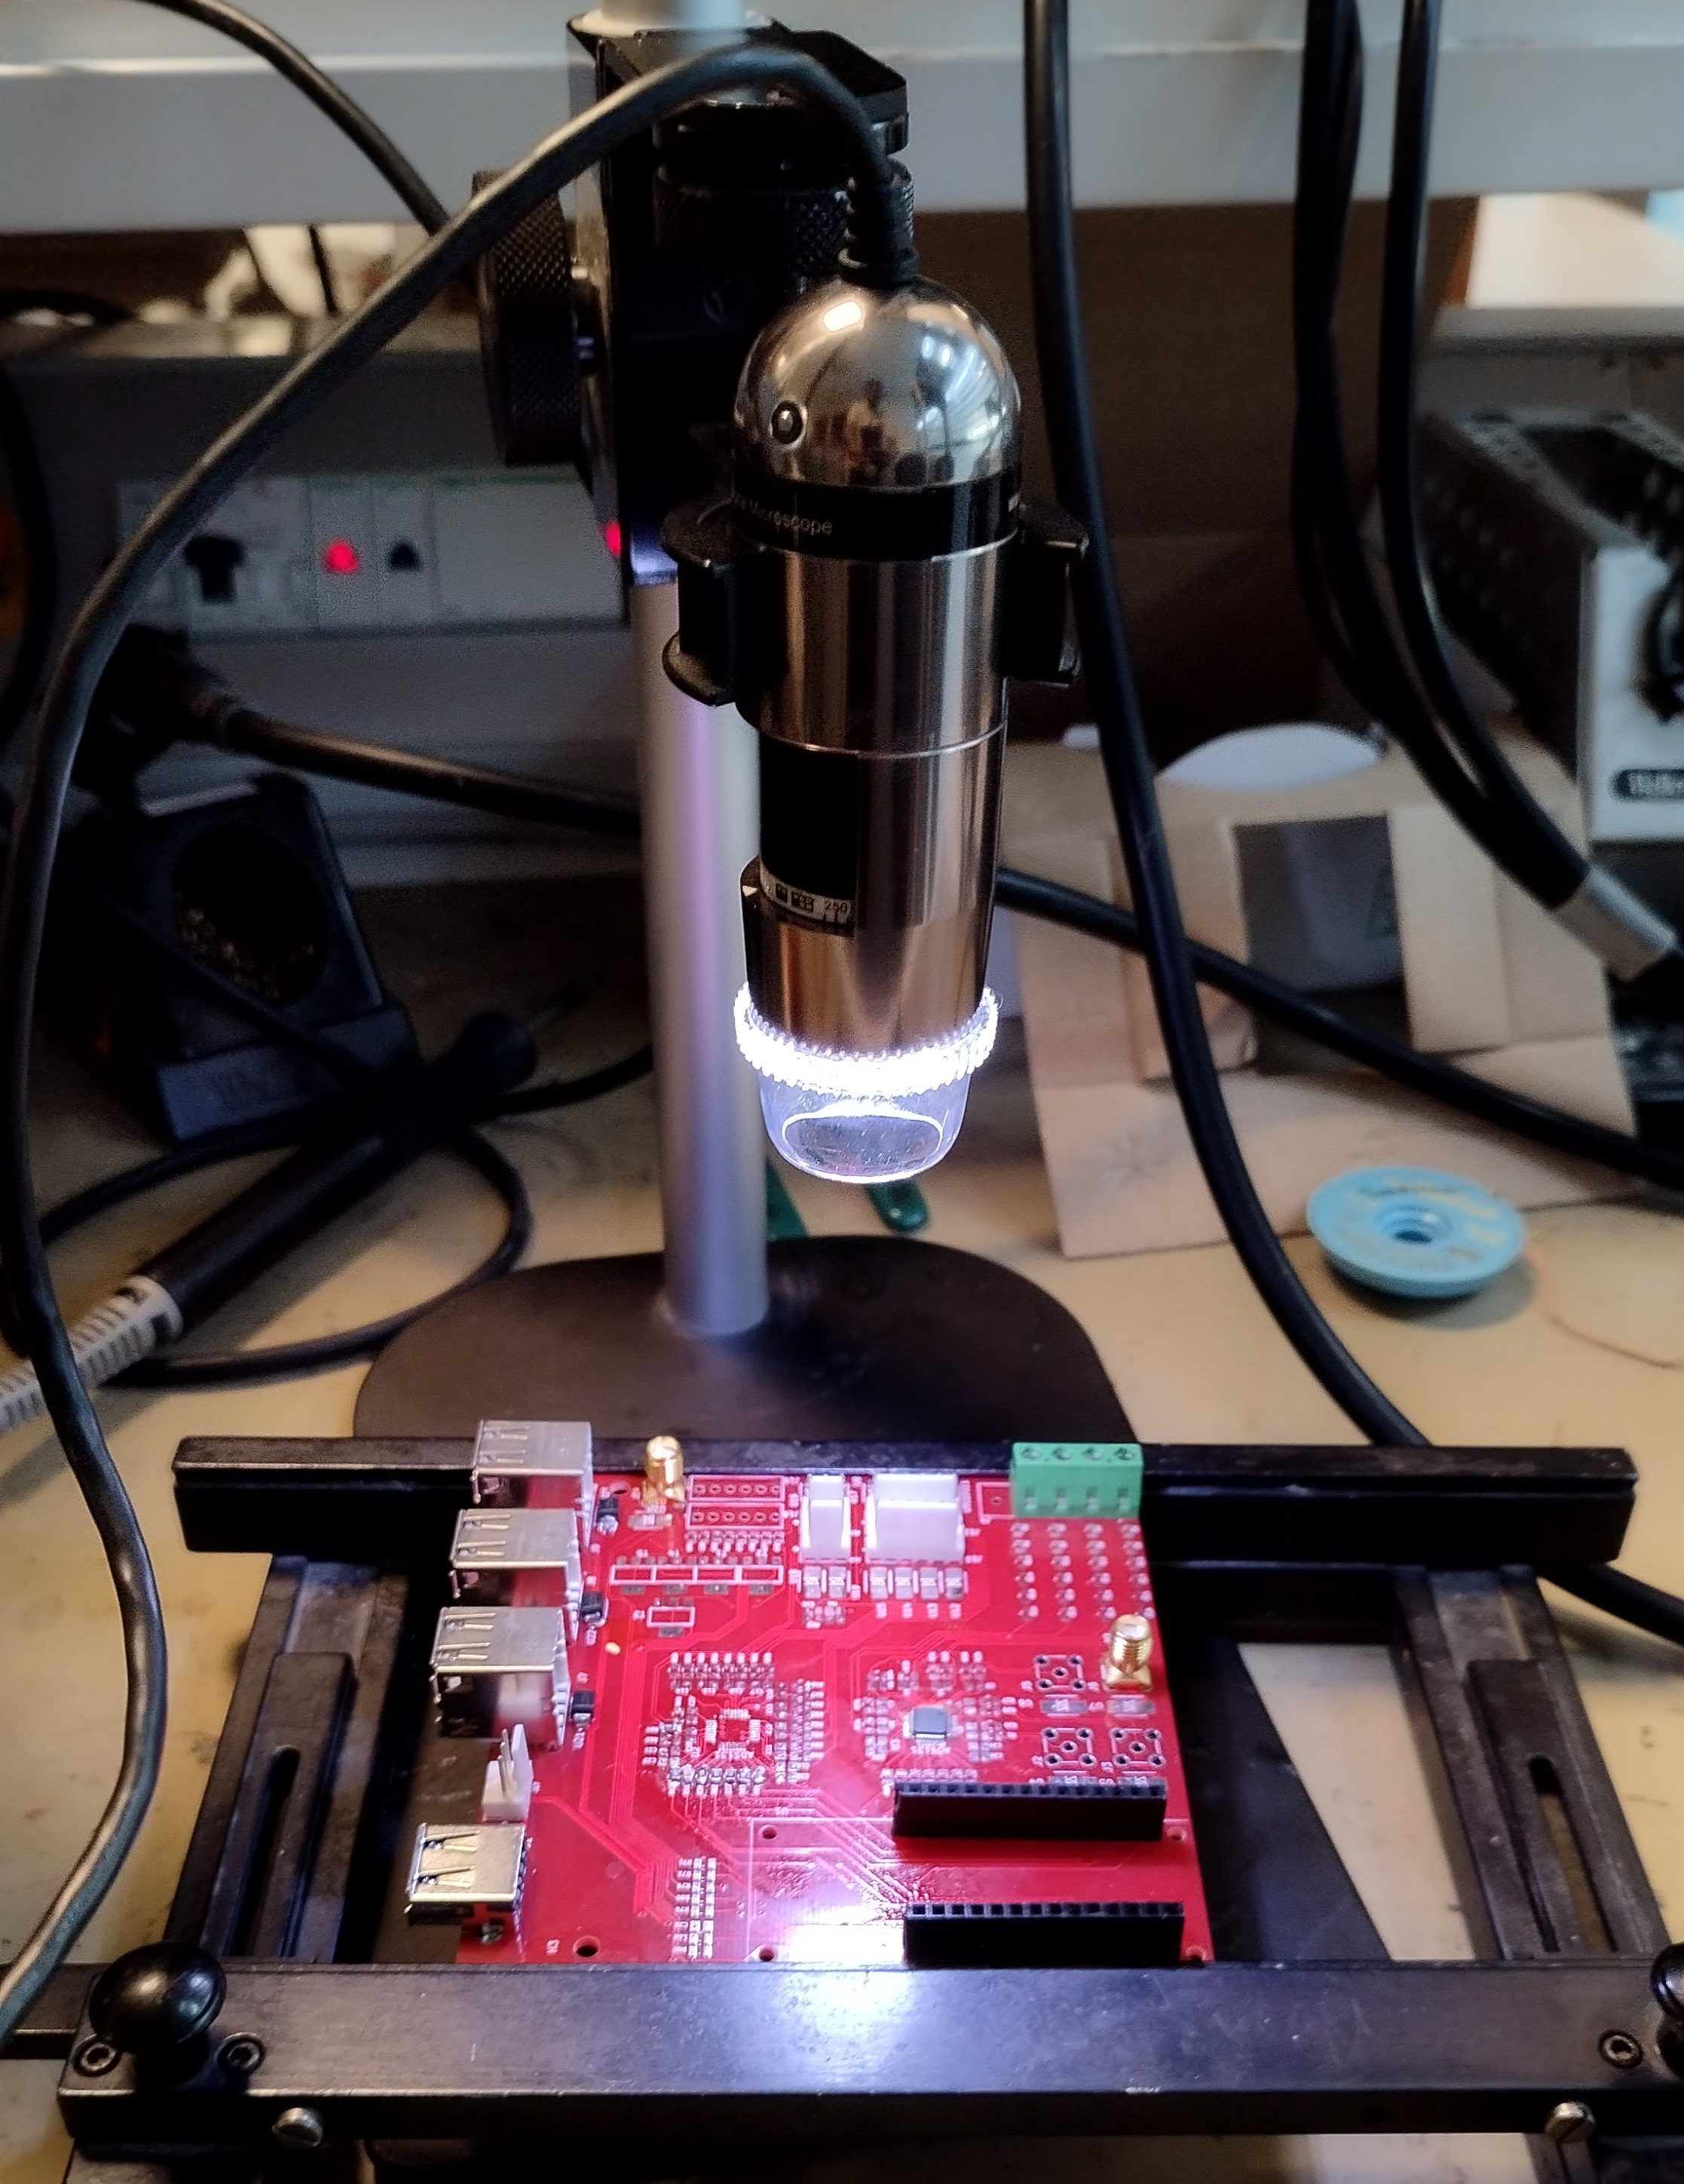
\includegraphics[scale=0.063]{images/Microscope.jpg}
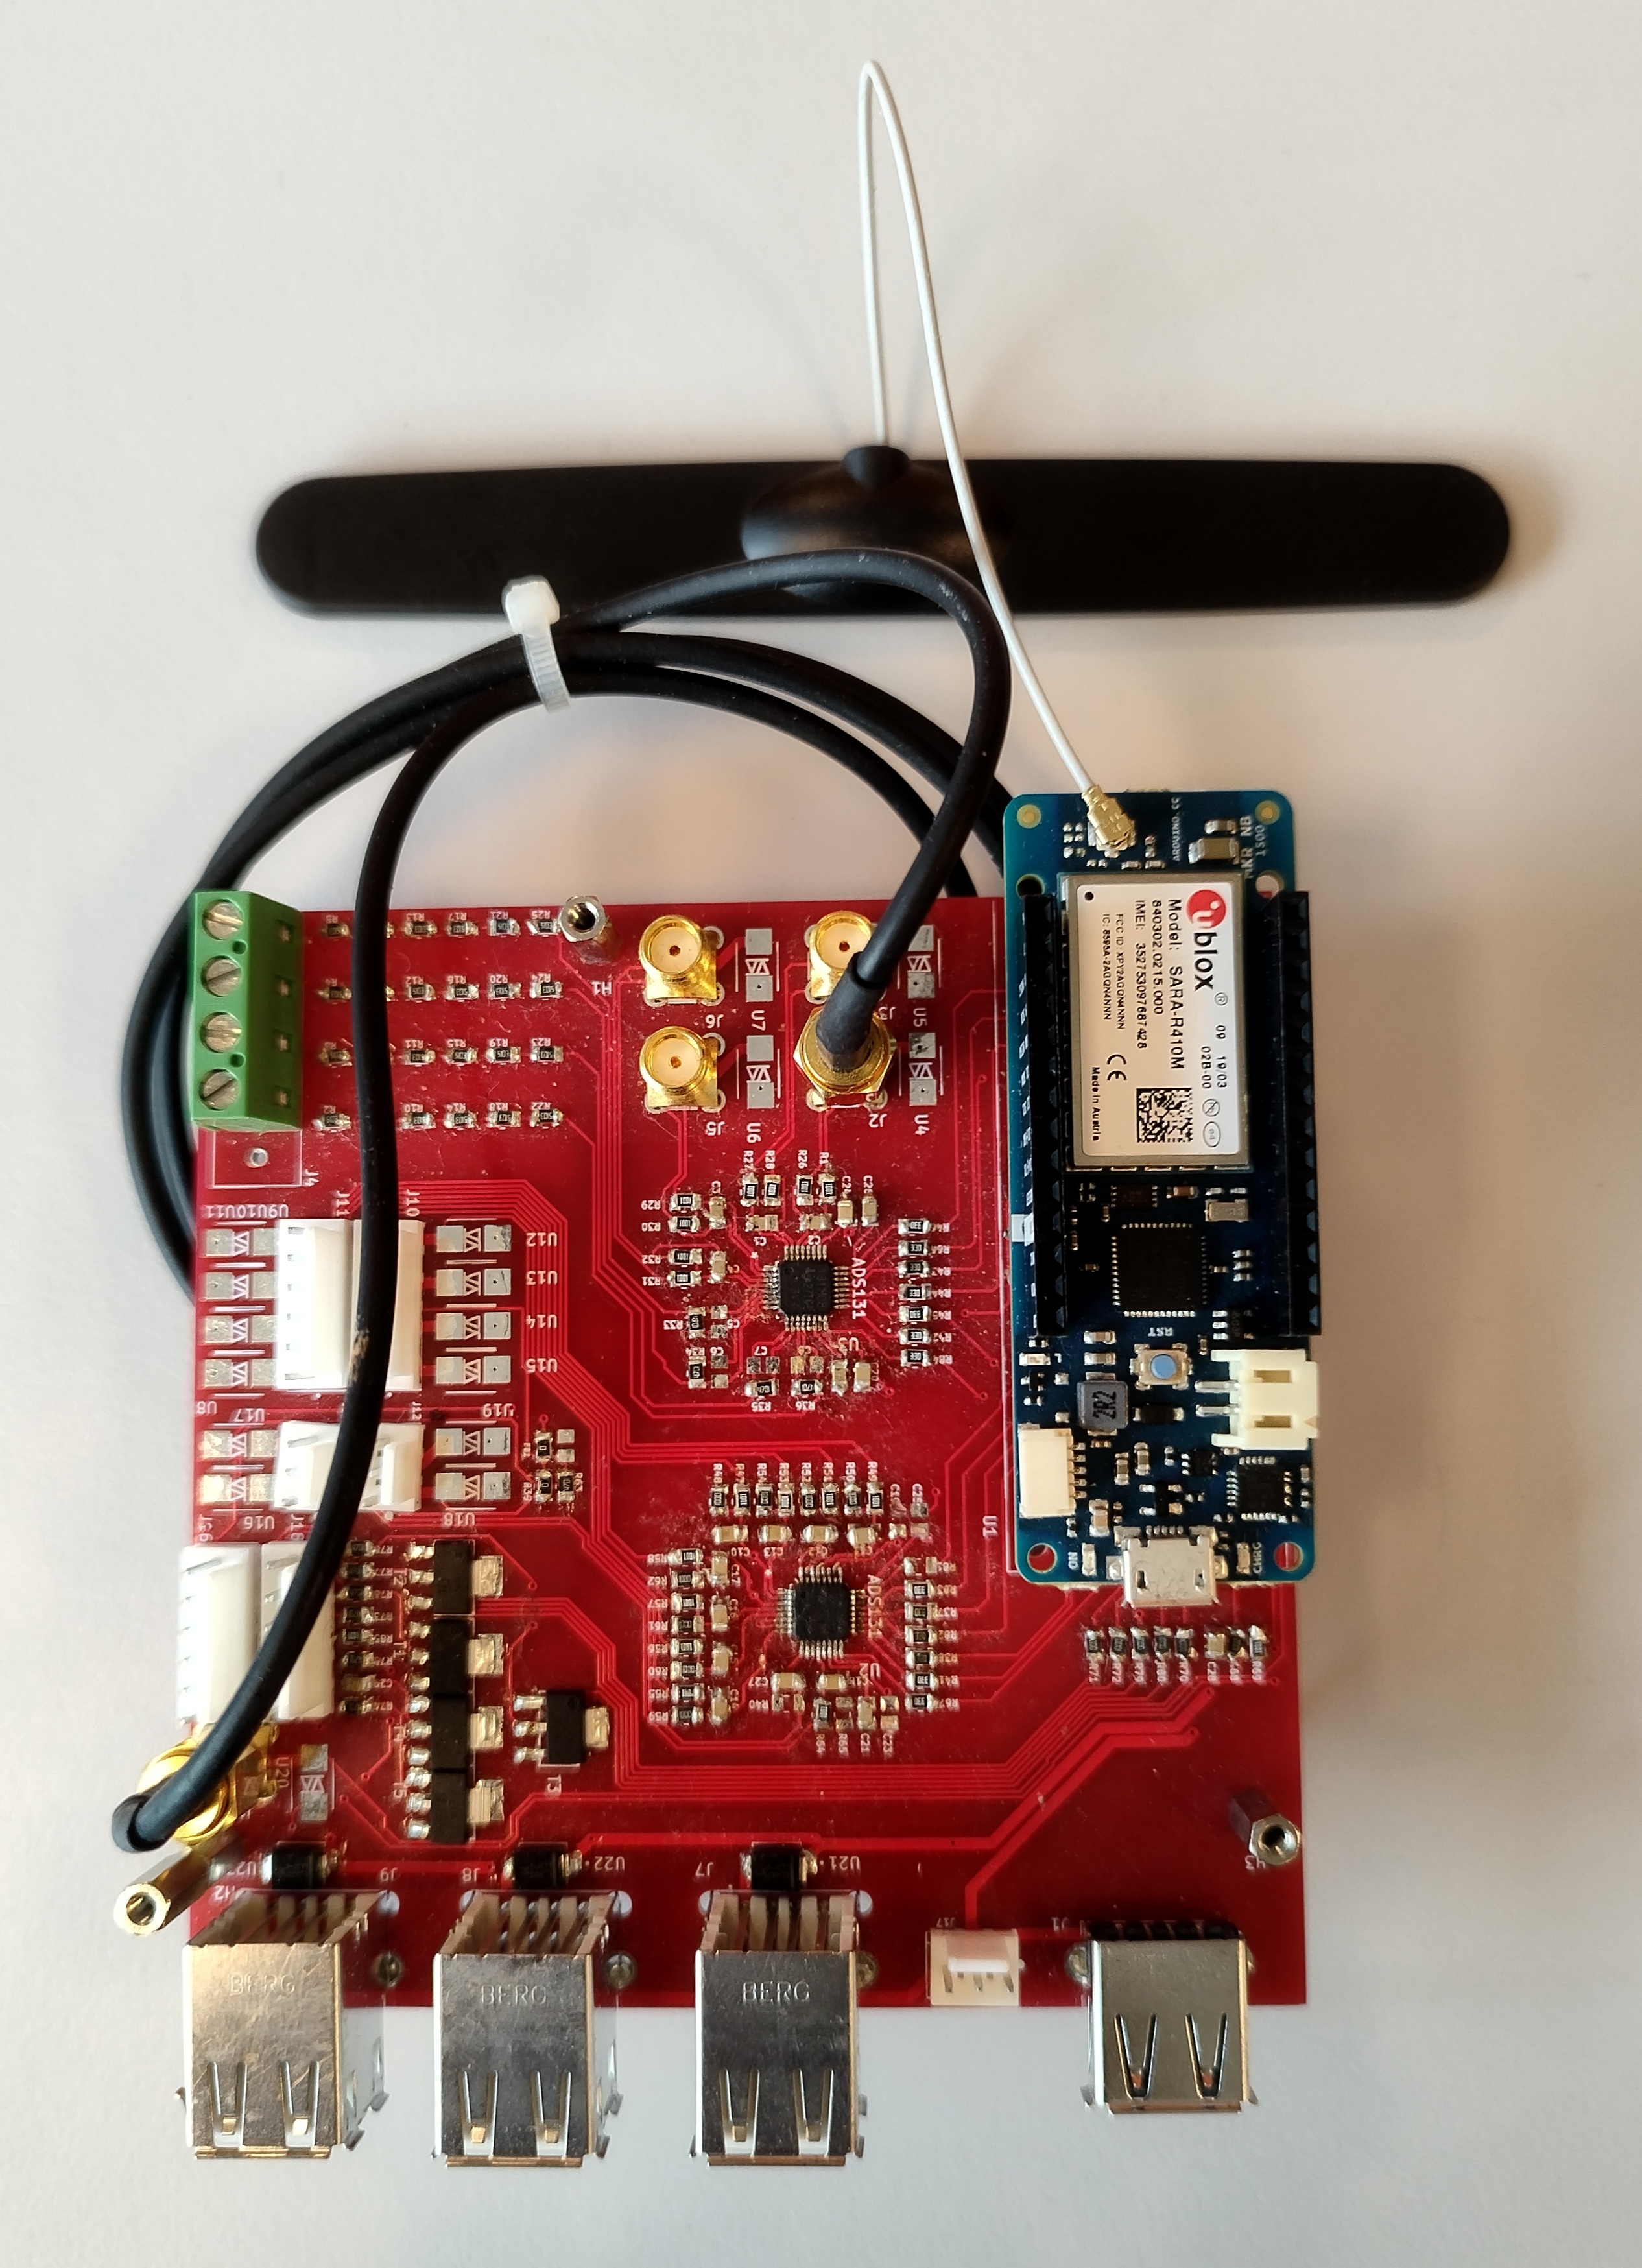
\includegraphics[scale=0.0525]{images/Board.jpg}
\caption{PCB Inspection and Implemented Board}
\label{fig:x Implemented Board}
\end{figure}
\textbf{Inspection and Testing:}  
 After soldering, the assembled PCBs undergo inspection to detect and correct any manufacturing defects such as solder bridges, missing components, or incorrect placements. Automated optical inspection (AOI) and X-ray machines are commonly used for this purpose. We have used Dino-Lite Edge AM73115MTF USB microscope for the inspection purpose shown in figure \ref{fig:x Implemented Board}. The final ready-to-run acquisition board also has been shown in the right figure.
\par

\nomenclature{$API$}{Application Programming Interface}
\nomenclature{$RMS$}{Root Mean Square}
\nomenclature{$PGA$}{Programmable Gain Amplifier}
\nomenclature{$KSPS$}{Kilo Samples Per Second}
\nomenclature{$SPI$}{Serial Peripheral Interface}
\nomenclature{$XTAL$}{Crystal}
\nomenclature{$PCB$}{Printed Circuit Board}
\nomenclature{$LP$}{Low Power}
\nomenclature{$VLP$}{Very Low Power}